\chapter{阳极氧化锡的生长模型和多孔氧化锡的电容性能}

\section{研究现状分析}
当今，纳米二氧化锡材料在染料敏化太阳能电池、气体传感器、锂离子电池、光电催化等领域具有潜在的应用价值……

\section{实验过程}
\subsection{纳米多孔氧化锡层的合成}
锡箔（纯度99.99\%，厚度100$\mu$m）作为阳极氧化的起始材料……

\section{结果与讨论}
\subsection{用于分析氧化锡形态的双电流模型}
图2.1显示了低电压（3-5V）下600s阳极氧化纳米管的表面和横截面电镜图像。从图2.1a可以观察到……

\begin{figure}[htbp]
    \centering
    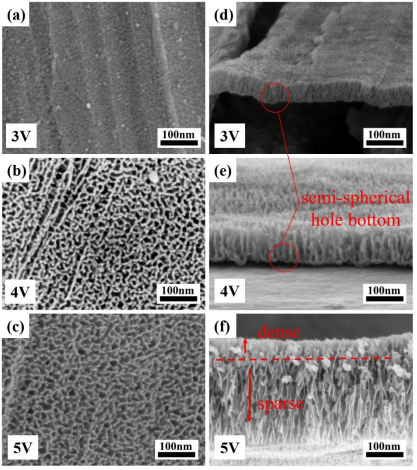
\includegraphics[width=0.6\textwidth]{fig/ch2/图片1.png}
    \caption[实验装置示意图]{阳极氧化锡在0.25M NaOH中，在3V（a，d），4V（b，e）和5V（c，f）下阳极氧化10min后的SEM图像，俯视图（a−c）和横断面图（d−f）}
    \label{fig:sem_sn}
\end{figure}

由表2.1可以看出，$R_{ct}$随着沉积时间的延长逐渐降低……

\begin{table}[H]
    \centering
    \caption[聚丙烯中空纤维主要性能指标]{MG$_{ratio}$ 在不同沉积时间下电化学参数的模拟得到的 EIS 结果}
    \label{tab:eis_results}
    \setlength{\tabcolsep}{0pt}
    \setlength{\aboverulesep}{0pt} % 清空横线上方的自动间距
    \setlength{\belowrulesep}{0pt} % 清空横线下方的自动间距
    \begin{tabular}{c c}
        \toprule[0.5bp]
        \rule{0pt}{0.8375cm} \makebox[6.05cm][c]{样本} & \makebox[8.88cm][c]{$R_{L} (\Omega \cdot \text{cm}^{-2})$} \\
        \midrule[0.5bp]
        \rule{0pt}{0.8375cm} \makebox[6.05cm][c]{MG4(500s)} & \makebox[8.88cm][c]{0.564} \\
        \rule{0pt}{0.8375cm} \makebox[6.05cm][c]{MG4(1000s)} & \makebox[8.88cm][c]{0.539} \\
        \rule{0pt}{0.8375cm} \makebox[6.05cm][c]{MG4(1500s)} & \makebox[8.88cm][c]{0.564} \\
        \bottomrule[0.5bp]
    \end{tabular}
\end{table}